\documentclass[12pt]{article}
\usepackage[margin=0.5in,top=0.5in,bottom=0.5in]{geometry}
\usepackage{amsmath}
\usepackage{indentfirst}
\usepackage{scrextend}
\usepackage{graphicx}
\usepackage{wrapfig}
\graphicspath{{images/}}

\title{\textbf{\underline{Assignment 3 Report}}}
\author{Anoop (2015CS10265)}

\begin{document}
\pagenumbering{gobble}
\maketitle

\section*{\underline{Decision Trees}}
\subsection*{Decision Tree Implementation}
\begin{addmargin}[0.3in]{0in}
\begin{tabbing}
Number of Nodes \qquad \= = 7972 \\
Train Accuracy \> = 0.88933 \\
Validation Accuracy \> = 0.79933 \\
Test Accuracy  \> = 0.80671 \\
\end{tabbing}
\end{addmargin}
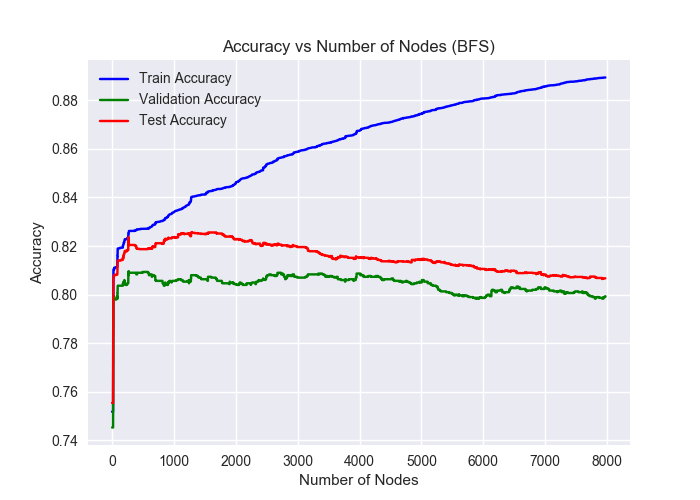
\includegraphics[width=0.5\textwidth]{dtree1.png}
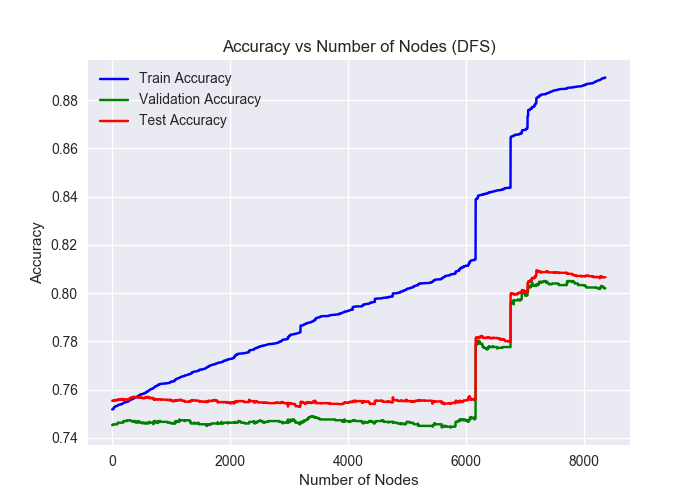
\includegraphics[width=0.5\textwidth]{dtree2.png}
\vspace{1mm}
\begin{addmargin}[0.3in]{0in}
From both BFS and DFS ways of growing the decision tree, we can observe that the training accuracy increases with number of nodes. Also from the validation and test accuracy curves we can say that the decision tree is overfitting the data. The decision tree is not able to fit the data completely because of the pre-processing that has been done on the data (There are examples where for the same features, the labels are different).
\end{addmargin}
\subsection*{Post-Pruning}
\begin{addmargin}[0.3in]{0in}
\begin{tabbing}
Number of Nodes \qquad \= = 2322 \\
Train Accuracy \> = 0.84893 \\
Validation Accuracy \> = 0.83467 \\
Test Accuracy  \> = 0.82557 \\
\end{tabbing}
\end{addmargin}
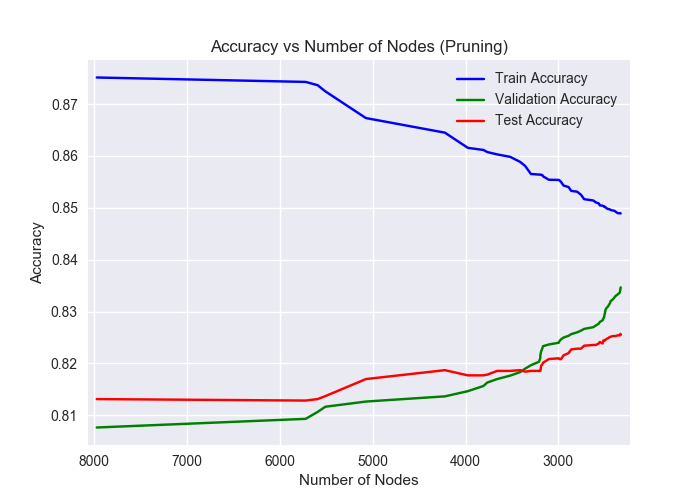
\includegraphics[width=0.5\textwidth]{dtree3.png}
\vspace{1mm}
\begin{addmargin}[0.3in]{0in}
From the graph, we can observe that post-pruning is reducing the overfitting. Also, as the validation accuracy is increasing, the test accuracy is also increasing.
\end{addmargin}
\subsection*{Decision Tree Implementation (Handling numerical features)}
\begin{addmargin}[0.3in]{0in}
\begin{tabbing}
Number of Nodes \qquad \= = 16495 \\
Train Accuracy \> = 0.99989 \\
Validation Accuracy \> = 0.78800 \\
Test Accuracy  \> = 0.77914 \\
\end{tabbing}
\end{addmargin}
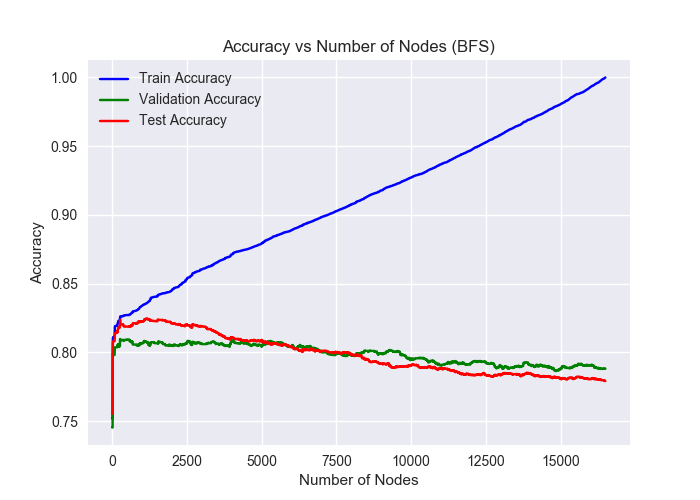
\includegraphics[width=0.5\textwidth]{dtree4.png}
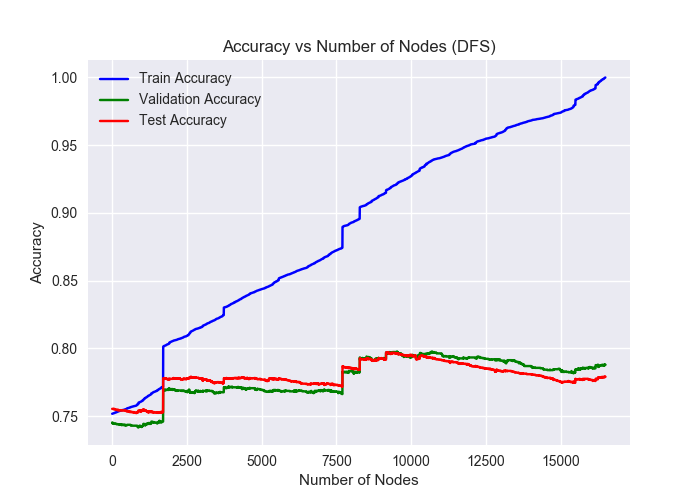
\includegraphics[width=0.5\textwidth]{dtree5.png}
\vspace{1mm}
\begin{addmargin}[0.3in]{0in}
In this modified implementation of decision trees, we are better able to handle numerical attributes. This can be seen in the training accuracy which is close to 100\%. The decision tree has almost completely fit the training data. This overfitting has brought down the validation and test accuracies.
\end{addmargin}
\vspace{2mm}
\begin{addmargin}[0.3in]{0in}
\begin{table}[h!]
\begin{center}
\caption{\underline{Number of splits per numerical feature}}
\vspace{1mm}
\label{tab:table1}
\begin{tabular}{|c|c|c|c|c|c|}
\hline
\textbf{Age} & \textbf{Fnlwgt} & \textbf{Education Number} & \textbf{Capital Gain} & \textbf{Capital Loss} & \textbf{Hour per Week} \\
\hline
3446 & 2194 & 0 & 18 & 6 & 536 \\
\hline
\end{tabular}
\end{center}
\end{table}
\end{addmargin}
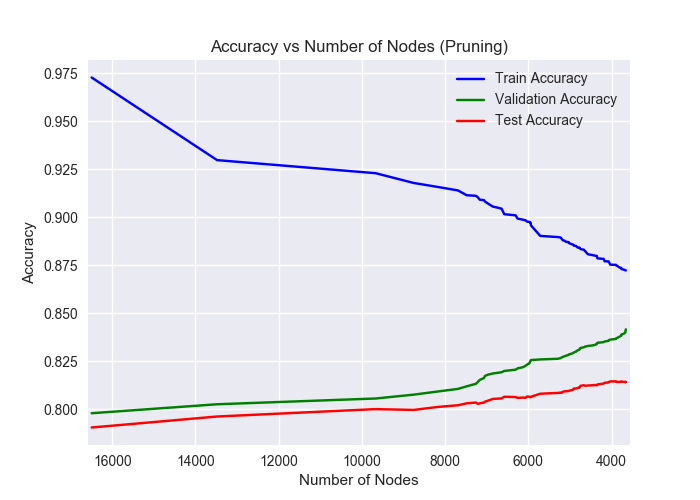
\includegraphics[width=0.5\textwidth]{dtree6.png}
\begin{addmargin}[0.3in]{0in}
\begin{tabbing}
Number of Nodes \qquad \= = 3650 \\
Train Accuracy \> = 0.87230 \\
Validation Accuracy \> = 0.84167 \\
Test Accuracy \> = 0.81429 \\
\end{tabbing}
\vspace{-3mm}
\end{addmargin}
\begin{addmargin}[0.3in]{0in}
Post-Pruning the fully grown decision tree (modified) gives even better validation accuracy but lesser test accuracy.
\end{addmargin}
\subsection*{Decision Tree Implementation - Scikit-Learn}
\vspace{-7mm}
\begin{table}[h!]
\begin{center}
\caption{\underline{Best Parameters (from 2160 models)}}
\vspace{1mm}
\label{tab:table2}
\begin{tabular}{|c|c|c|c|c|c|}
\hline
\textbf{Model} & \textbf{criterion} & \textbf{max\_depth} & \textbf{min\_samples\_split} & \textbf{min\_samples\_leaf} & \textbf{max\_features} \\
\hline
1 & gini & 12 & 0.005 & 0.001 & None \\
2 & entropy & 10 & 0.005 & 0.001 & None \\
\hline
\end{tabular}
\end{center}
\end{table}
\vspace{-13mm}
\begin{table}[h!]
\begin{center}
\caption{\underline{Accuracies}}
\vspace{1mm}
\label{tab:table3}
\begin{tabular}{|c|c|c|c|}
\hline
\textbf{Model} & \textbf{Train Accuracy} & \textbf{Validation Accuracy} & \textbf{Test Accuracy} \\
\hline
1 & 0.83507 & 0.82633 & 0.82914 \\
2 & 0.83574 & 0.82633 & 0.83000 \\
\hline
\end{tabular}
\end{center}
\end{table}
\vspace{-5mm}
\begin{addmargin}[0.3in]{0in}
\textbf{max\_depth} restricts the depth of the decision tree, \textbf{min\_samples\_split} restricts the splitting of small nodes and \textbf{min\_samples\_leaf} enforces a minimum size requirement for a node to be a leaf. All these hyperparameters help in reducing overfitting. As compared to greedy post-pruning, these hyperparameters need to be tuned manually. In this case, searching for the hyperparameters helps rather than greedy post-pruning marginally (over test accuracies).
\end{addmargin}
\subsection*{Random Forest Implementation - Scikit-Learn}
\vspace{-7mm}
\begin{table}[h!]
\begin{center}
\caption{\underline{Best Parameters (from 17280 models)}}
\vspace{1mm}
\label{tab:table2}
\begin{tabular}{|c|c|c|c|c|c|c|c|}
\hline
\textbf{Model} & \textbf{criterion} & \textbf{n\_estimators} & \textbf{max} & \textbf{min} & \textbf{min} & \textbf{max} & \textbf{bootstrap} \\
&  &  & \textbf{\_depth} & \textbf{\_samples} & \textbf{\_samples} & \textbf{\_features} & \\
&  &  &  & \textbf{\_split} & \textbf{\_leaf} &  & \\
\hline
1 & gini & 2 & 8 & 0.01 & 1 & 10 & False\\
2 & entropy & 2 & 12 & 0.01 & 0.001 & 10 & True\\
\hline
\end{tabular}
\end{center}
\end{table}
\begin{table}[h!]
\begin{center}
\caption{\underline{Accuracies}}
\vspace{1mm}
\label{tab:table3}
\begin{tabular}{|c|c|c|c|}
\hline
\textbf{Model} & \textbf{Train Accuracy} & \textbf{Validation Accuracy} & \textbf{Test Accuracy} \\
\hline
1 & 0.83263 & 0.82867 & 0.82586 \\
2 & 0.83119 & 0.82933 & 0.82771 \\
\hline
\end{tabular}
\end{center}
\end{table}
\vspace{-5mm}
\begin{addmargin}[0.3in]{0in}
\textbf{n\_estimators} specifies the number of decision trees in the random forest , \textbf{max\_features} restricts the number of features searched over while choosing the split and \textbf{bootstrap} specifies if bootstrap samples are used or not. As compared to greedy post-pruning, these hyperparameters need to be tuned manually. In this case also, searching for the hyperparameters helps rather than greedy post-pruning marginally (over test accuracies).
\end{addmargin}

\section*{\underline{Neural Networks}}

\end{document}